\documentclass[a4paper]{abntex2}
\usepackage[T1]{fontenc}
\usepackage{graphicx}
\usepackage{amsmath}
\usepackage{multicol,multirow}
\usepackage[bottom=2.5cm,top=2.5cm,left=2.0cm,right=2.0cm]{geometry}
\usepackage{indentfirst}
\usepackage{hyperref}  %%%%
\hypersetup{colorlinks,citecolor=black,filecolor=blacke,linkcolor=blue,urlcolor=blue} %%%%
\renewcommand\thesection{\arabic{section}} % não inclui capítulo na mumeração da seção
\setcounter{page}{0} % não conta a numeração da capa
\pagestyle{myheadings} %numerar página sem títulos extras
\usepackage[abnt-emphasize=bf,alf,bibjustif,versalete]{abntex2cite}
\usepackage{lipsum} % pacote para escrever texto aleatório.

\usepackage{xcolor}
\usepackage{here}
\usepackage{hyperref}

\usepackage{tabularx}   % para tabelas ajustáveis
\usepackage{booktabs}   % para linhas mais bonitas
\usepackage{array} % Para opções de formatação de colunas / formatar colunas

\usepackage{listings}
% Configurando o estilo global do Java
\lstset{
  language=Java,
  basicstyle=\ttfamily\small,      % Fonte e tamanho do código
  keywordstyle=\color{blue},      % Cor das palavras-chave (ex: public, class, static)
  commentstyle=\color{gray},      % Cor dos comentários
  stringstyle=\color{red},        % Cor das strings (ex: "Hello, World!")
  showstringspaces=false,         % Não mostrar espaços em strings de forma especial
  numbers=left,                   % Numerar linhas à esquerda
  numberstyle=\tiny\color{gray},  % Estilo dos números de linha
  breaklines=true,                % Quebrar linhas longas automaticamente
  frame=single,                   % Adicionar uma moldura ao redor do código
  captionpos=b                    % Posição da legenda (b=bottom)
}

\begin{document}

% --- Inclusão da capa ---
% --- capa.tex ---

\begin{center}
%\hspace{-0.5cm}
\raisebox{-2\baselineskip}{
\includegraphics[width=0.15\textwidth]
{imagens/logo-uenf.png}}
\hfill
\begin{minipage}[b]{0.80\textwidth}
  \textbf{\Large Universidade Estadual do Norte Fluminense Darcy Ribeiro}\\
  \centering
    \textbf{\Large Centro de Ciência e Tecnologia}\\
  %\textbf{\large Paradigma Orientado a Objetos para Desenvolvimento de Software}
\end{minipage}
\vspace{200pt}

        \huge{\textbf{Projeto POO Dev}}\\ %Entre aqui com título
        \Large{Sistema para o Pescarte}\\ %Entre com o subtítulo
        
        \vspace{150pt}
        
        \vspace{40pt} 

        \hfill Arthur Cézar Martins Ferreira Mól \hspace{20pt} Matrícula: 20221100108\\

        \vspace{25pt}
        \hfill {Professor: João Luiz de Almeida Filho}\\ 
     
        \vspace{\fill}
        \LARGE \textbf{\today}
          
	\end{center}


%% o índice remissivo pode ser retirado se excluir o texto desde esse comentário até a próxima sequência de %, não se esqueça também de excluir os hyperref lá no alto, estarão marcados com símbolos.
\newpage

%\Large\tableofcontents
%\thispagestyle{empty}
             %%%%%
%\newpage


\tableofcontents % Gera o sumário

\newpage % Garante que o sumário termine e o próximo conteúdo comece em uma nova página

\section{GitHub}

\href{https://github.com/arthurcezarmol/projeto-POO-Dev}{Clique aqui} para ser redirecionado ao repositório onde o projeto está.

\section{Descrição do sistema}

Linguagem para o back-end (e orientação a objetos) \textbf{Java} utilizando o framework \textbf{Springboot}.

Para o front-end será usado \textbf{React}.

Para o banco de dados será usado \textbf{Postgree}.

O sistema que será criado é uma plataforma interativa para o projeto PEA-Pescarte. O intuito desse sistema é criar uma plataforma onde os pescadores artesanais que participam do projeto possam logar, interagir com a plataforma e utilizar os serviços que serão fornecidos pela plataforma, como o de controle de gastos e lucro, além de informações gerais.

O sistema visa buscar fornecer serviços aos pescadores artesanais de modo a facilitar a vida deles, além de torná-los mais conectados.

As funcionalidades que estarão presentes no sistema são: 

\begin{itemize}
    \item Página \textbf{Home}: contendo as informações principais e mais relevantes do momento no site;
    \item Página \textbf{Login}: contendo a tela de login e criação de conta;
    \item Página \textbf{Serviços}: contendo serviços que podem vir a ser relevantes para os pescadores, como indicações de lojas como fábricas de gelo, lojas de artigos de pesca, informações sobre transporte, serviço de mecânico para os barcos;
    \item Página \textbf{Clima}: contendo informações sobre a previsão do tempo para o dia, se existe possibilidade de chuva, velocidade do vento, dentre outros;
    \item Página \textbf{Financeiro}: que faz um "controle" do financeiro dos pescadores, nessa página eles vão poder inserir o que pescaram e a aplicação vai fazer uma estimativa de por quanto eles deveriam vender os peixes baseado em informações estaduais e federais. Além disso, também uma opção de gerar uma planilha financeira com os gastos e lucros dos mesmos;
    \item Página \textbf{Sobre}: essa página vai conter as informações sobre o que é o projeto PEA-Pescarte.
\end{itemize}

\subsection{O que é o projeto PEA-Pescarte}

O Projeto PESCARTE tem como sua principal finalidade a criação de uma rede social regional integrada por pescadores artesanais e por seus familiares, buscando, por meio de processos educativos, promover, fortalecer e aperfeiçoar a sua organização comunitária e a sua qualificação profissional, bem como o seu envolvimento na construção participativa e na implementação de projetos de geração de trabalho e renda.

O Projeto de Educação Ambiental Pescarte (PEA Pescarte) trabalha junto às \textbf{comunidades de pesca artesanal} de Arraial do Cabo, Búzios, Cabo Frio, Campos, Carapebus, Macaé, Rio das Ostras, Quissamã, São Francisco de Itabapoana e São João da Barra. Desde 2014, atua juntamente aos pescadores artesanais e seus familiares, por meio de processos educativos, promovendo, fortalecendo e aperfeiçoando a organização comunitária e a sua qualificação profissional, bem como o seu envolvimento na construção participativa e na implementação de projetos de geração de trabalho e renda.

O processo educativo é realizado nos 10 municípios e se dá através de oficinas com temas diversos, entre eles: economia solidária, cooperativismo, políticas públicas, licenciamento ambiental, letramento digital e gestão participativa. O projeto promove, também, articulações entre os pescadores e pescadoras, com reuniões do Grupo de Trabalho, Grupo Gestor, Grupo de Acompanhamento de Obras e assembleias municipais.

\section{Requisitos funcionais e não funcionais}

\subsection{Requisitos funcionais}

Definem a \textbf{funcionalidade} que o sistema a ser desenvolvido deverá ter. Ele é um requisito relacionado com um tipo de comportamento produto de uma função do sistema.

Os requisitos funcionais deste projeto são:

\begin{itemize}
    \item Cadastrar usuários;
    \item Realizar login;
    \item Transmitir dados;
    \item Exibir informações do usuário;
    \item Mostrar serviços;
    \item Gerar documentos;
    \item Consultar documentos.
\end{itemize}

Os requisitos funcionais se relacionam diretamente a processos\footnote{processos = verbos} que o sistema deve executar. Ex: pesquisar, cadastrar, relatar, verificar, imprimir.

\subsection{Requisitos não-funcionais}

Indicam propriedades comportamentais que o sistema deve possuir.

Os requisitos não-funcionais deste sistema são:

\begin{itemize}
    \item Poder acessar a aplicação usando qualquer navegador;
    \item Poder acessar a aplicação usando qualquer dispositivo: celular, tablet ou computador (responsividade);
    \item Aplicação com informações expostas de modo que pessoas com dificuldade de usar elementos da tecnologia possa acessá-lo sem problemas (acessibilidade com botões e textos grandes e intuitivos);
    \item Boa formatação, legibilidade e confiabilidade dos documentos gerados pelo sistema;
    \item Usuários poderem fazer login somente atrelados a uma Corporativa.
\end{itemize}

\section{Diagrama de classes inicial}

\subsection{Diagrama de classes (UML)}

\begin{figure}[H]
    \centering
    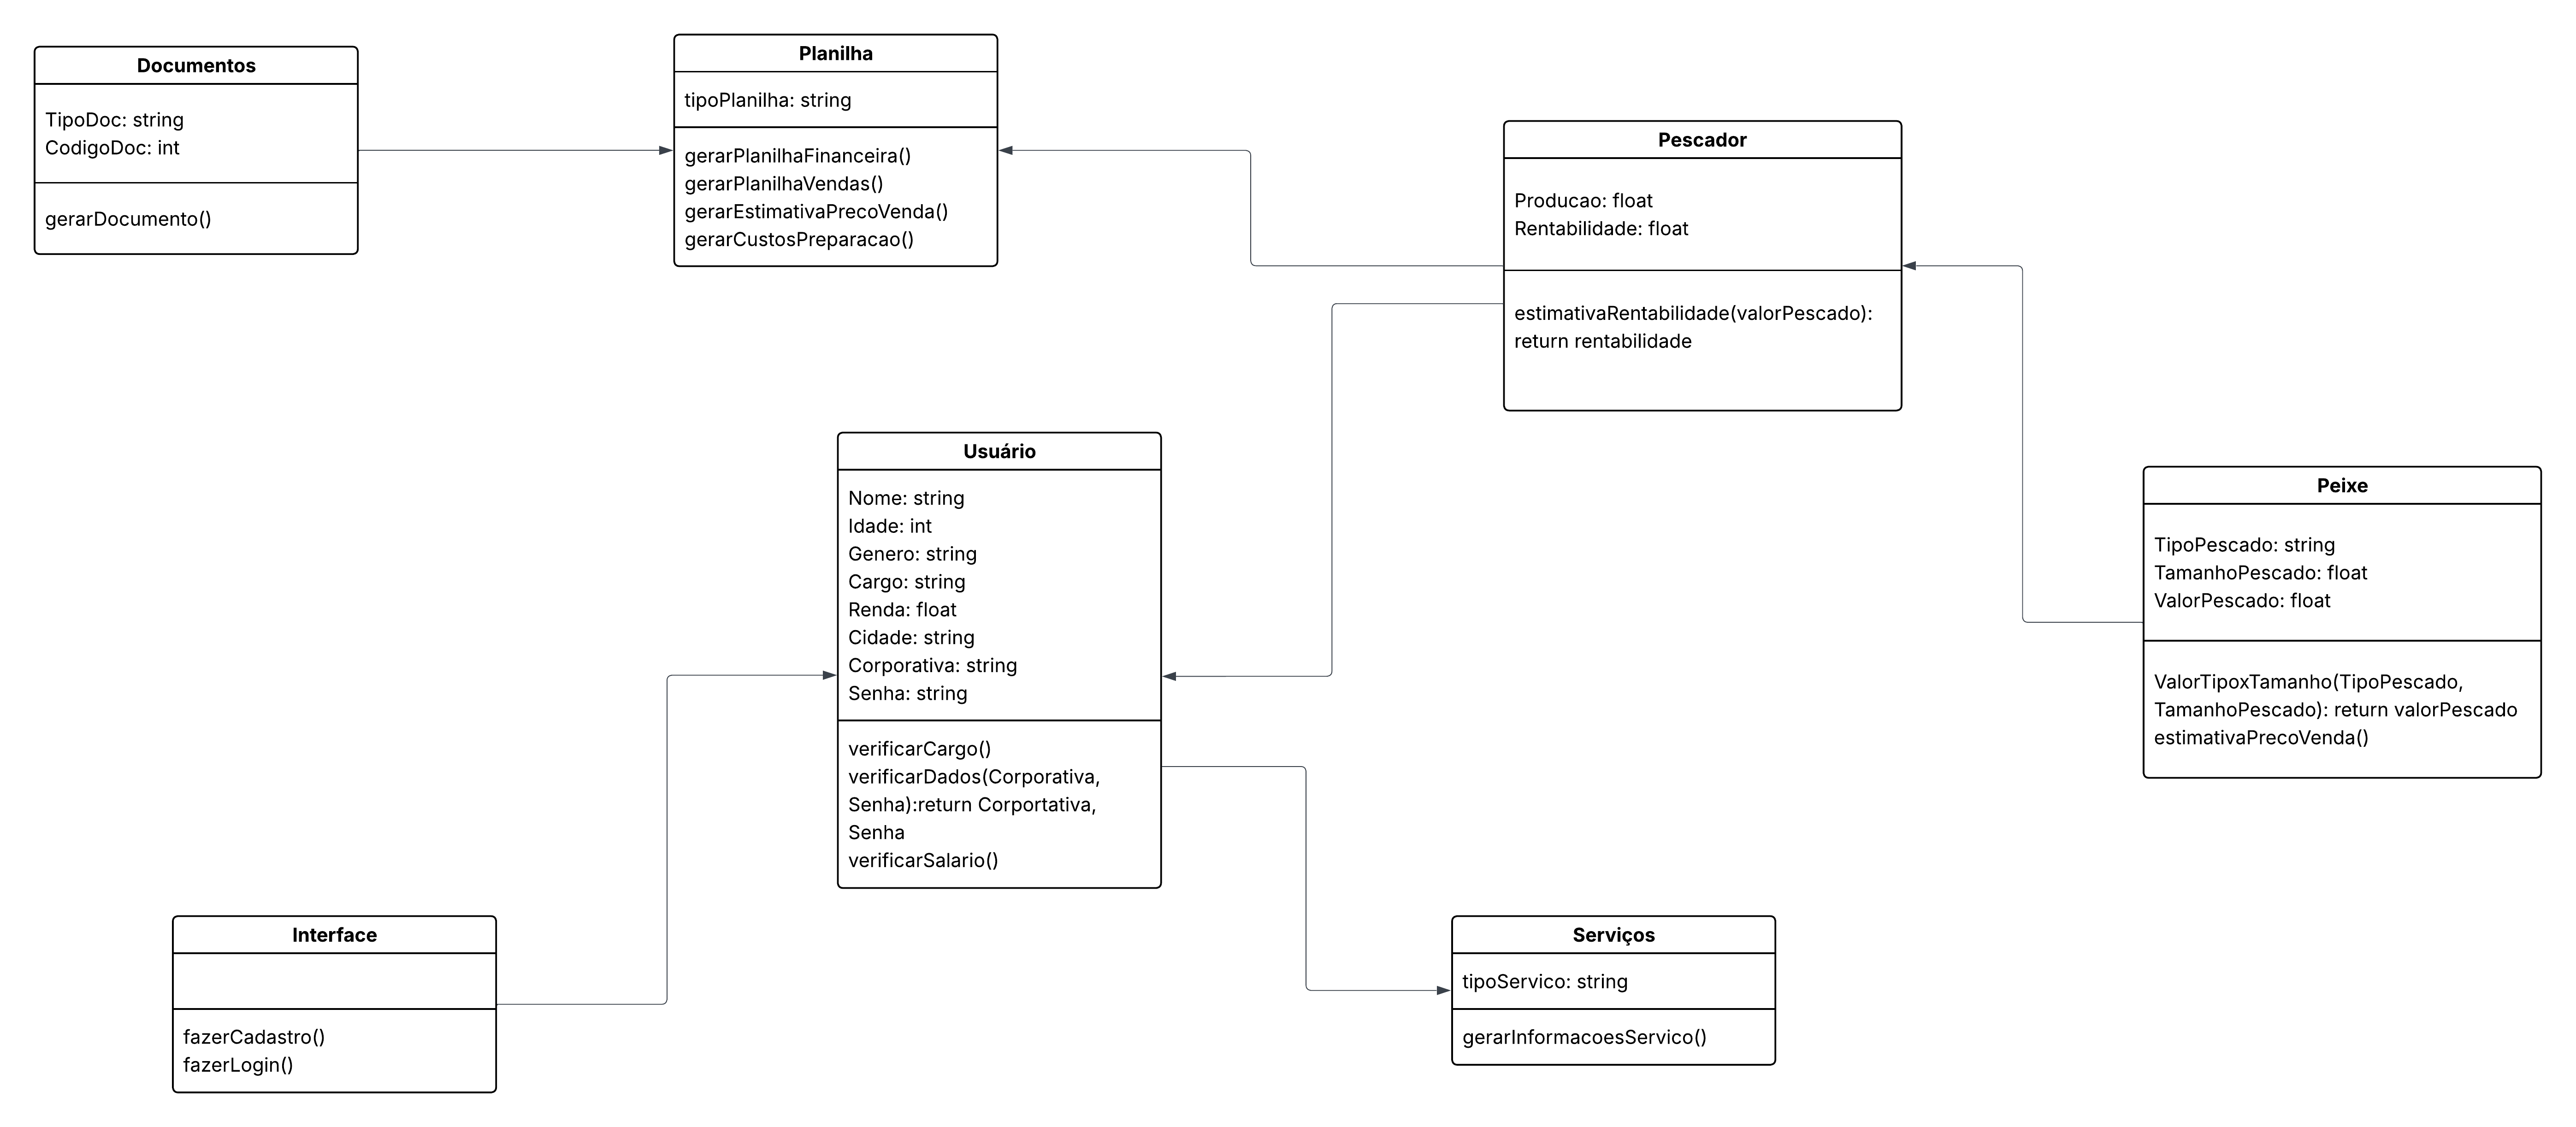
\includegraphics[width=1\linewidth]{imagens/UML POO DEV.png}
    \caption{Diagrama UML do projeto}
    \label{fig:uml-projeto}
\end{figure}

\subsection{Diagrama entidade relacionamento (ER)}

\begin{figure}[H]
    \centering
    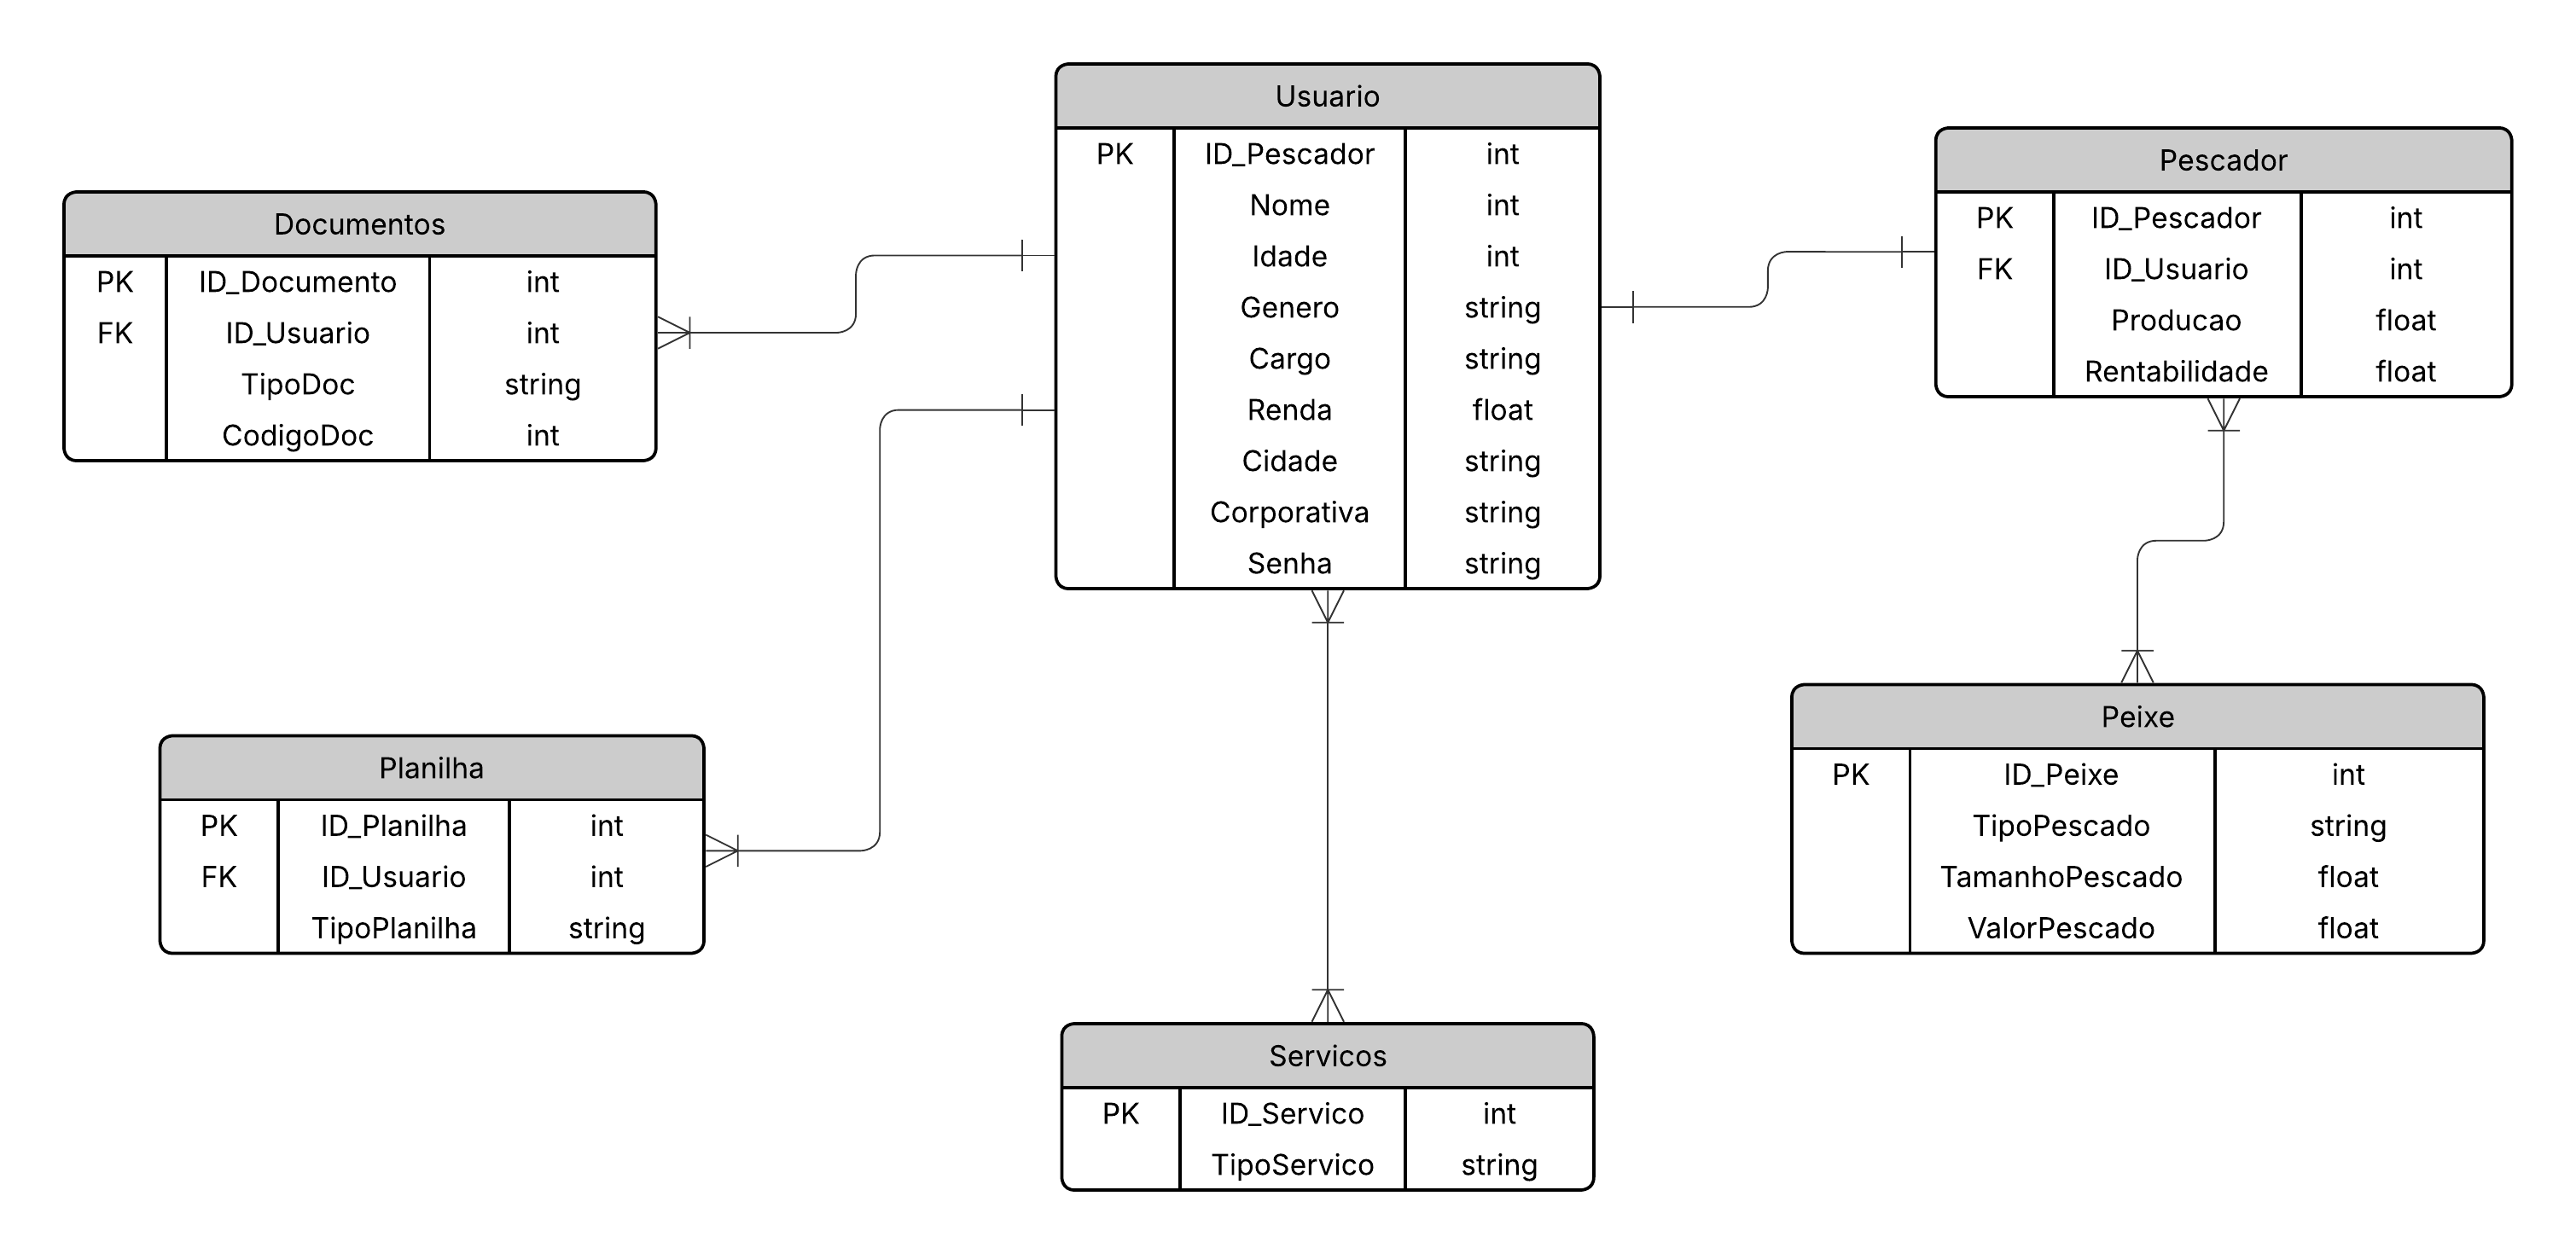
\includegraphics[width=1\linewidth]{imagens/Diagrama ER de banco de dados.png}
    \caption{Diagrama ER do projeto}
    \label{fig:er-projeto}
\end{figure}

\section{Fluxo básico de funcionamento}

\subsection{Diagrama de casos de uso}

\begin{figure}[H]
    \centering
    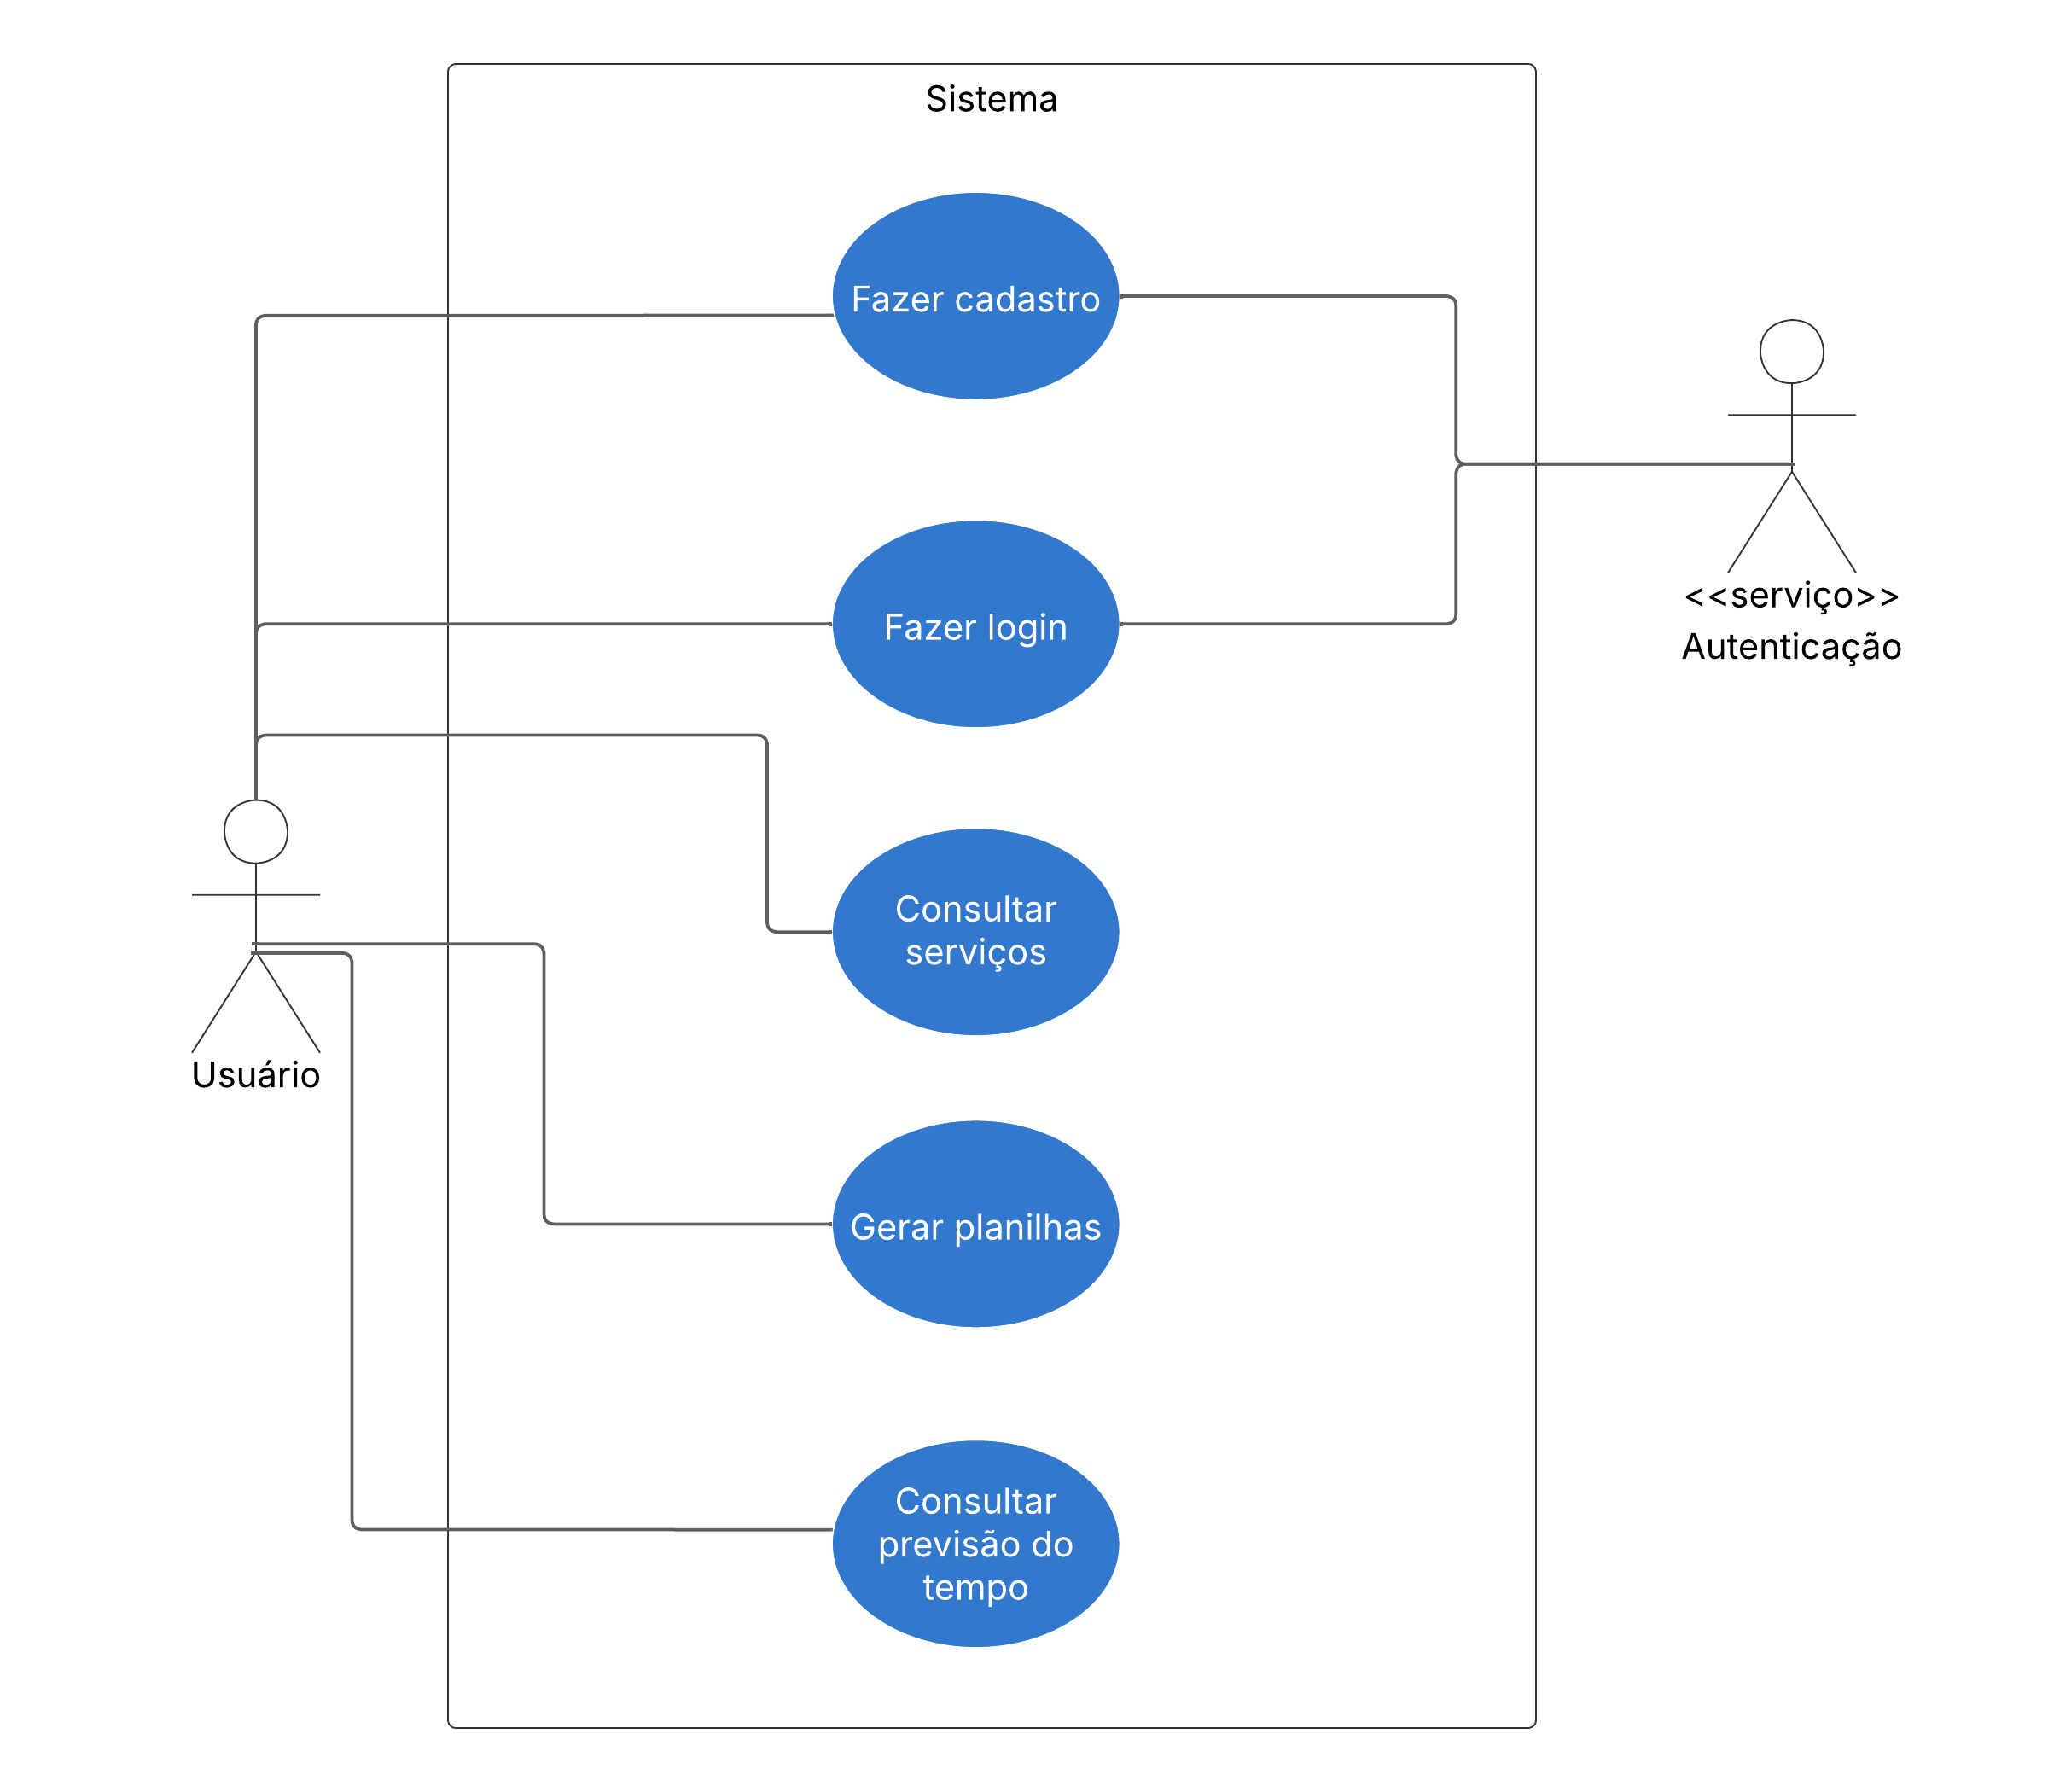
\includegraphics[width=1\linewidth]{imagens/Caso de Uso POO DEV.png}
    \caption{Diagrama de Casos de Uso do projeto}
    \label{fig:casos-de-uso-projeto}
\end{figure}

\section{Orçamento}

\subsection{Custo do desenvolvimento}

Cobrando R\$100,00 a hora. Por dia seriam utilizadas pelo menos 2 horas de trabalho, considerando que seriam trabalhados 5 dias da semana no mínimo 1 hora durante 3 meses, o custo final do desenvolvimento seria por volta de R\$3000,00.

\subsection{Custo de manutenção}

Mensalmente seria cobrado o custo mensal da hospedagem do site, que seria cerca de R\$300,00. Além do custo mensal de manutenção, que seria cerca de 2 horas de trabalho por mês exclusivamente para manutenção, o que sairia cerca de R\$200,00. Resultando um total de R\$500,00 mensais.

\subsection{Custo total}

O preço total do projeto sairia pelo preço total R\$3000,00 mais R\$500,00 por mês que o cliente continuar contratando os serviços de manutenção.

\section{Cronograma detalhado por semana}

\begin{table}[h!]
\centering
\renewcommand{\arraystretch}{1.3} % aumenta espaçamento entre linhas
\begin{tabularx}{\textwidth}{>{\bfseries}c c X}
\toprule
Semana & Datas & Atividade \\
\midrule
1  & 15/09 -- 19/09 & Planejamento do modelo do front-end \\
2  & 22/09 -- 26/09 & Criação do esqueleto do front-end \\
3  & 29/09 -- 03/10 & Planejamento e criação do banco de dados \\
4  & 06/10 -- 10/10 & Planejamento do modelo do back-end \\
5  & 13/10 -- 17/10 & Criação do back-end \\
6  & 20/10 -- 24/10 & Aprimoramento do back-end \\
7  & 27/10 -- 31/10 & Aprimoramento do back-end \\
8  & 03/11 -- 07/11 & Aprimoramento do front-end \\
9  & 10/11 -- 14/11 & Aprimoramento do front-end \\
10 & 17/11 -- 21/11 & Conexão entre front-end, back-end e banco de dados \\
11 & 24/11 -- 28/11 & Revisão geral e melhorias pontuais \\
12 & 01/12 -- 03/12 & Entrega do projeto pronto \\
\bottomrule
\end{tabularx}
\caption{Cronograma de desenvolvimento do projeto}
\end{table}

\section{Realização do projeto}

Nesta seção irei detalhar o cumprimento ou não cumprimento das tarefas propostas na seção 7.

\subsection{Primeira semana}

\textbf{Objetivo}: Planejamento do modelo front-end

\textbf{Realizado}: Foi feito um wireframe (figura \ref{fig:wireframe-projeto}) para representar uma base de como o site vai ser. Um wireframe é um esboço visual básico e de baixa fidelidade de um site ou aplicativo, que ilustra a estrutura e o layout de uma página ou tela.

\begin{figure}[H]
    \centering
    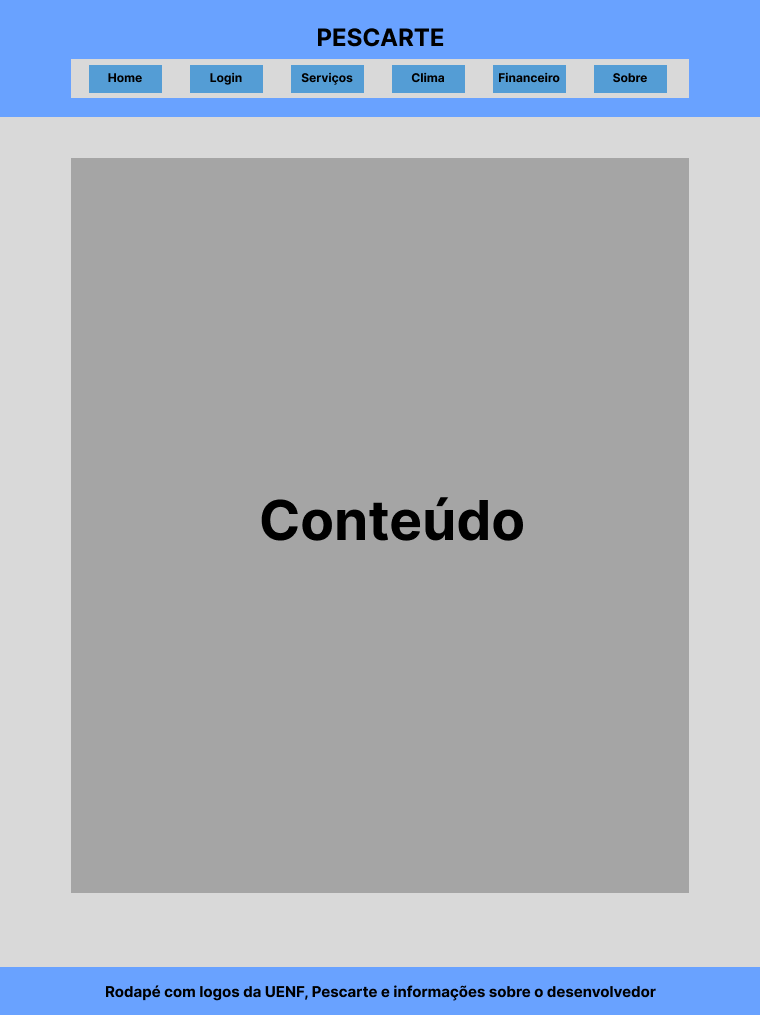
\includegraphics[width=0.75\linewidth]{imagens/Wireframe-projeto.png}
    \caption{Wireframe do projeto}
    \label{fig:wireframe-projeto}
\end{figure}

Além disso, também foi feito o que foi proposto para a Semana 2: foram criadas as pastas iniciais do projeto (Figura \ref{fig:esqueleto-front-end}) e também foi criada uma estrutura inicial para o front-end, contendo uma NavBar funcional, que altera as páginas das seções do site corretamente e os conteúdos principais de cada página (Figura \ref{fig:estrutura-inicial-projeto}).

\begin{figure}[H]
    \centering
    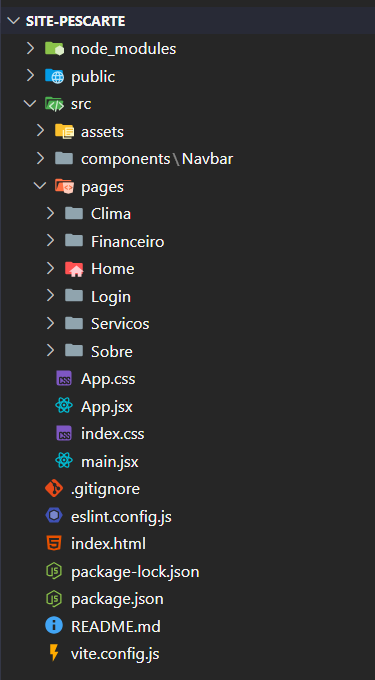
\includegraphics[width=0.25\linewidth]{imagens/esqueleto-front-end.png}
    \caption{Estrutura inicial das pastas do projeto}
    \label{fig:esqueleto-front-end}
\end{figure}

\begin{figure}[H]
    \centering
    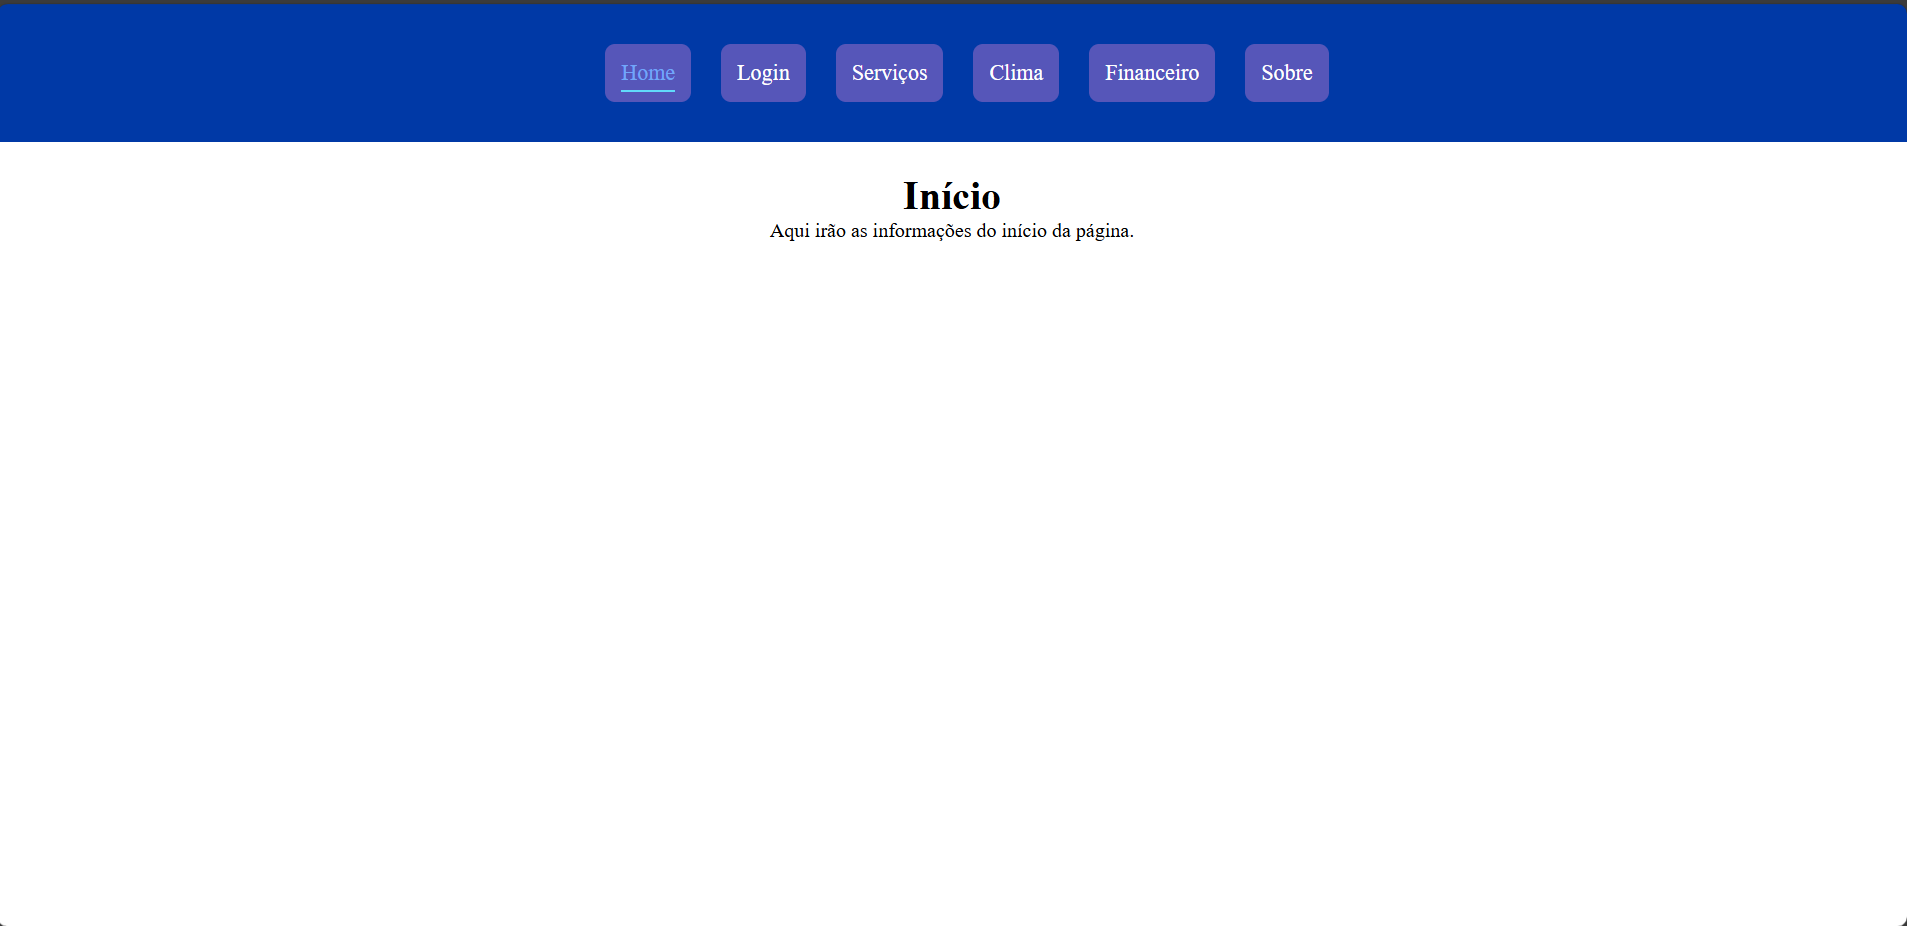
\includegraphics[width=1.0\linewidth]{imagens/estrutura-inicial-projeto.png}
    \caption{Estrutura inicial do site}
    \label{fig:estrutura-inicial-projeto}
\end{figure}

\subsection{Segunda semana}

\textbf{Objetivo}: Criação do esqueleto do front-end

\textbf{Realizado}: O que foi proposto na segunda semana já foi realizado na primeira. Na segunda semana nada foi feito em detrimento à semana de provas.

\subsection{Terceira semana}

\textbf{Objetivo}: Planejamento e criação do banco de dados

\textbf{Realizado}: Foi atualizado o diagrama entidade relacionamento (Figura \ref{fig:er-projeto}). Além disso foi criada a estrutura base do banco de dados, com todas as tabelas e atributos (Figura \ref{fig:estrutura-banco-de-dados}).

\begin{figure}[H]
    \centering
    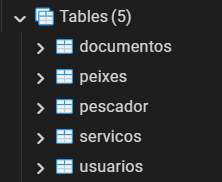
\includegraphics[width=0.5\linewidth]{imagens/estrutura-banco-de-dados.png}
    \caption{Estrutura do Banco de Dados}
    \label{fig:estrutura-banco-de-dados}
\end{figure}

\subsection{Quarta semana}

\textbf{Objetivo}: Planejamento do modelo do back-end

\textbf{Realizado}: Foi criada a estrutura do back-end, como é possível ver na figura \ref{fig:estrutura-back-end}.

\begin{figure}[H]
    \centering
    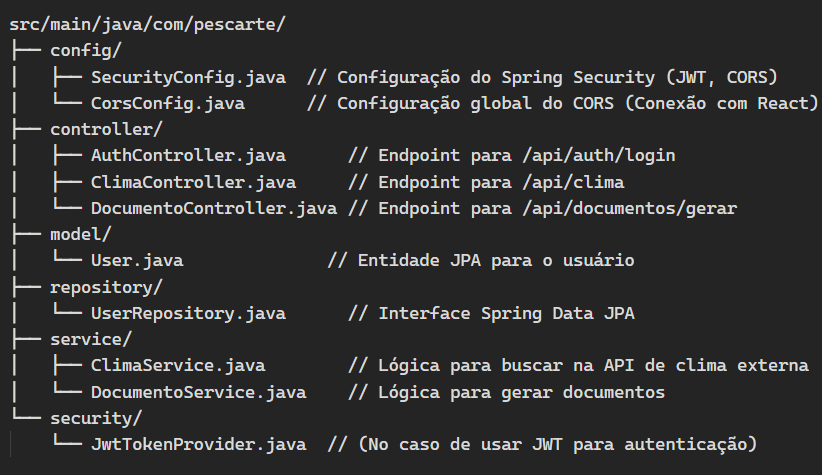
\includegraphics[width=0.9\linewidth]{imagens/estrutura-back-end.png}
    \caption{Estrutura do Back-end}
    \label{fig:estrutura-back-end}
\end{figure}

Além disso também foram criadas tuplas para começar a popular as tabelas do banco de dados.

\subsection{Quinta semana}

\textbf{ATRASO}

\subsection{Sexta semana}

\textbf{ATRASO}

\subsection{Sétima semana}

\textbf{Objetivo:} Aprimoramento do back-end

\textbf{Realizado:} Configuração da conexão do banco de dados com o back-end, como podemos no código \ref{code:config-bd}

\begin{lstlisting}[caption={Conexão banco de dados com back-end}, label={code:config-bd}]
// Configuracao do PostgreSQL
spring.datasource.driver-class-name=org.postgresql.Driver
spring.datasource.username=postgres
spring.datasource.password=190603
spring.datasource.url=jdbc:postgresql://localhost:5432/pescarte
spring.jpa.generate-ddl=true

// Configuracao do Hibernate (JPA)
spring.jpa.properties.hibernate.dialect=org.hibernate.dialect.PostgreSQLDialect
spring.jpa.hibernate.ddl-auto=update
spring.jpa.show-sql=true
\end{lstlisting}



\end{document}